% Created 2021-07-14 Wed 17:30
% Intended LaTeX compiler: xelatex
\documentclass[11pt]{article}
\usepackage{amsmath}
\usepackage{xltxtra}

%% Global (changing main font and mono font which is used in verbatim)
\setmainfont{Source Han Sans CN} % Font for the hole text
\setmonofont{AR PL UMing CN} % Font for verbatim

%% Locally (setting local variables)
\newfontfamily\ch[Mapping=tex-text]{HAN NOM A} 
%AR PL UMing CN : light font
%AR PL UKai TW MBE : drawn font (marked traces)
\DeclareTextFontCommand{\unifont}{\ch}

\usepackage{verbatim, fancyvrb}
\date{\today}
\title{A little guide of Chinese Mandarin fonts in \LaTeX}
\begin{document}

\maketitle
% \tableofcontents

\section{Preamble}
\label{sec:org9153cc4}
\subsection{Begin document with fontspec}
\label{sec:org4c87d9b}
\begin{verbatim}
\documentclass{article}
\usepackage{fontspec} %Font package
\end{verbatim}

\subsection{Declare font (in your system)}
\label{sec:org3c49420}
We can declare the command ch,
\begin{verbatim}
%% Preamble %%
\newfontfamily\ch[Mapping=tex-text]{HAN NOM A} 
%AR PL UMing CN : light font
%AR PL UKai TW MBE : drawn font (marked traces)
\DeclareTextFontCommand{\unifont}{\ch}
\end{verbatim}

\section{Call the function inside the document}
\label{sec:org9f0b2b6}

Examples of use {\verb+{\ch{语}}+}:{\ch{语}}.

\begin{verbatim}
\begin{document}
{\ch{你好我说汉语}}
\end{document}
\end{verbatim}

 $=$ {\ch{你好我说汉语}}

\clearpage
\section{Note}
\label{sec:org643caa5}
To know the name of the fonts installed in the system which render Mandarin, we can instal \texttt{forfont}, written in Rust. Then, call it in the shell,

\begin{verbatim}
$ fontfor -p 语
\end{verbatim}

It will open a webpage rendering and showing the fonts available in the system.

{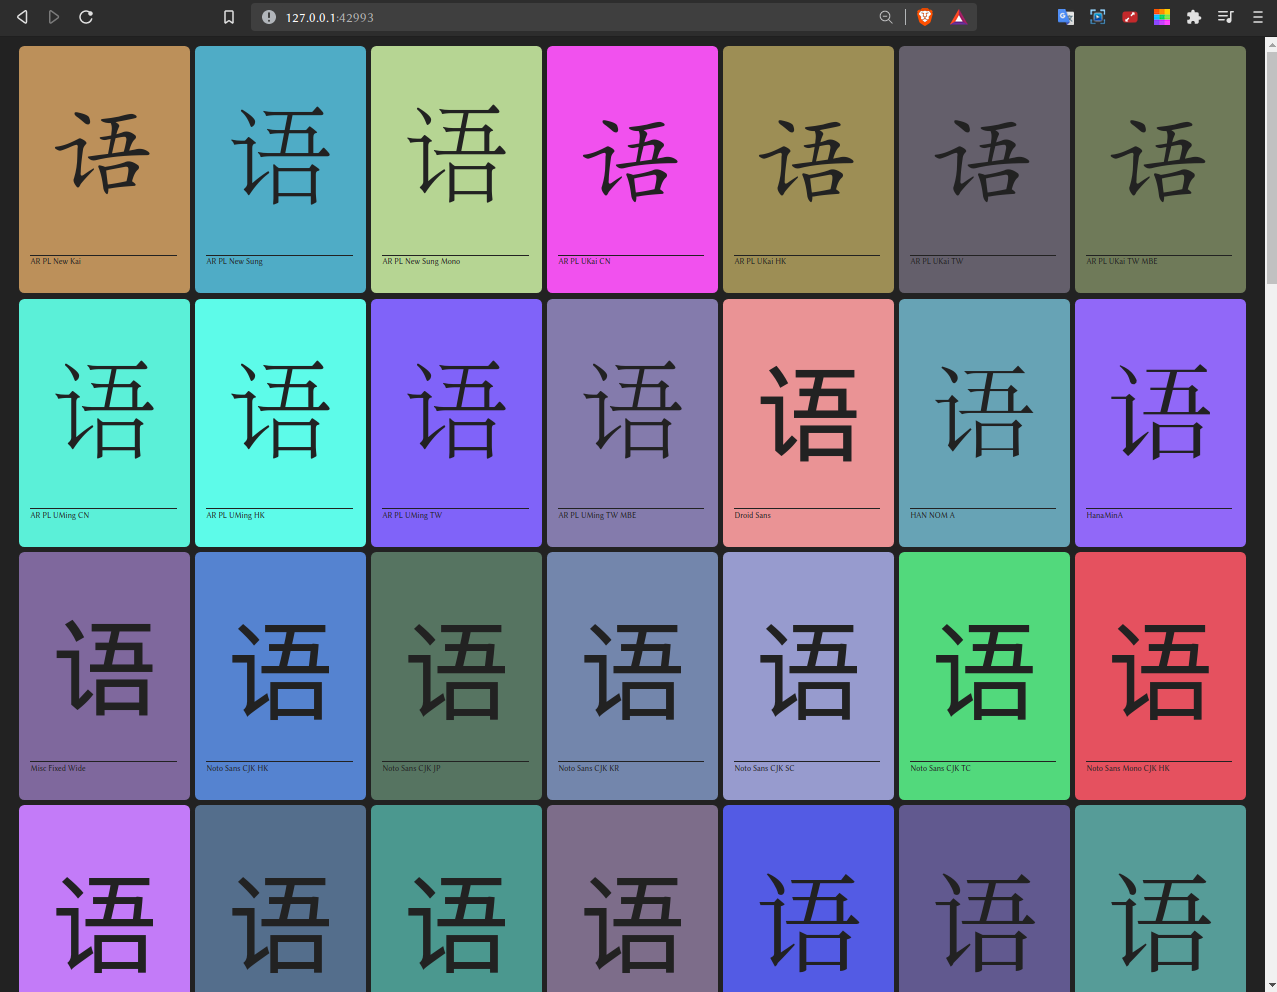
\includegraphics[width=.9\linewidth]{/home/buddhilw/PP/LaTeX/TCC/tests/pic-selected-210714-1454-51.png}}

Also, we can specify general fonts to be used in the hole document, also.

\begin{verbatim}
%% Preamble %%
\setmainfont{Source Han Sans CN} % Font for the hole text
\setmonofont{AR PL UMing CN} % Font for verbatim
\end{verbatim}
\end{document}